% !TEX root = ../../I4PRJ, Grp3 - Rapport.tex
\chapter{Proces og projektgennemførsel}

I afsnittet beskrives gennemførslen af projektet, herunder: udviklingmetode, processtyring, ledelse og værktøjer. Processen er vigtig ift. at opnå et godt resultat. 

\section{Proces}
Udviklingsmetoden for projektet er Scrum. Scrum er en agil udviklingsmetode \cite[kap. 1]{robertmartin2006}. Scrum er ikke indlemmet i processen i sin kanoniske form. I næste afsnit beskrives, hvordan projektprocessen afviger fra teorien.

\section{Scrum}
Scrum sprints er har været forlænget, da Scrum typisk bruges i fuldtids-udviklingteams, kunne det ikke lade sig gøre at have nok at samle op på efter en uges arbejde. Daglige Scrum meetings er blevet til ugentlige, spørgsmålene: Hvad har jeg lavet? Hvad mangler jeg at lave? Hvad skal der til, for at jeg kommer videre?, er blevet besvaret af hvert gruppemedlem. Den forlængede tid mellem møder har medført sprints har strukket sig over 2-3 uger af gangen. Med Scrum har gruppen forsøgt at være refleksiv over processen. Hvor spørgsmålene stilles; Hvad skal vi blive ved med at gøre? Hvad skal vi holde op med at gøre? Hvad skal vi begynde at gøre? På samme måde har gruppen reflekteret over processen og har eksempelvis løst følgende misforståelse og gjort gruppen opmærksom på øget kommunikation:

Der var gruppemedlemmer, som havde tendens til at arbejde på en del af systemet, uden at der var åbenhed omkring det. Det kunne have ført til evt. dobbelt arbejde, som ville have været spildt. Problemet blev bragt op tidligt i processen, hvormed gruppen har indgået konsensus om åbenhed af arbejdsopgaver, hvilket har gjort det nemmere at koordinere arbejde på tværs af undergrupper.

Gruppen har ikke anvendt den traditionelle rollefordeling i et Scrumteam. Alle gruppens medlemmer har været ligestillet som udviklere og rollerne som Scrum master og product owner har været en diskussion på møder, hvor demokratiske beslutninger er foretaget som erstatning. Til alle møder er der taget referat, og referent rollen er blevet udtrukket ved et hertil udviklet værktøj. Til alle møder er der blevet valgt en mødeleder, hvis ikke den bestemte mødeleder kunne være til mødet. Mødelederens rolle var ordstyrer og ansvar for overholdelse af dagsorden. 

For at holde styr på status i processen og i de enkelte sprints opererer Scrum med backlogs. Det er product backlog og sprint backlog, som i projektet er oprettet ved hjælp af værktøjet "Pivotal Tracker". 

\subsection{Pivotal Tracker}
Pivotal Tracker \url{pivotaltracker.com/} er et processtyringsværktøj, til projekter som bruger Scrum som udviklingsmetode. De forskellige backlogs i et Scrum projekt opstilles nemt og intuitiv i Pivotal. Pivotal benyttes story begrebet, hvilket har gjort det nemt at arbejde med user stories og manøvrerer user stories mellem stadier af udfærdigelse. De forskellige stadier af udfærdigelse såsom, i backlog, igangværende (sprint backlog) og færdig, har ageret scrumboard. 
 Figur~\ref{fig:scrumboard} viser et eksempel på gruppens Pivotal Tracker side.

\begin{figure}
	\centering
	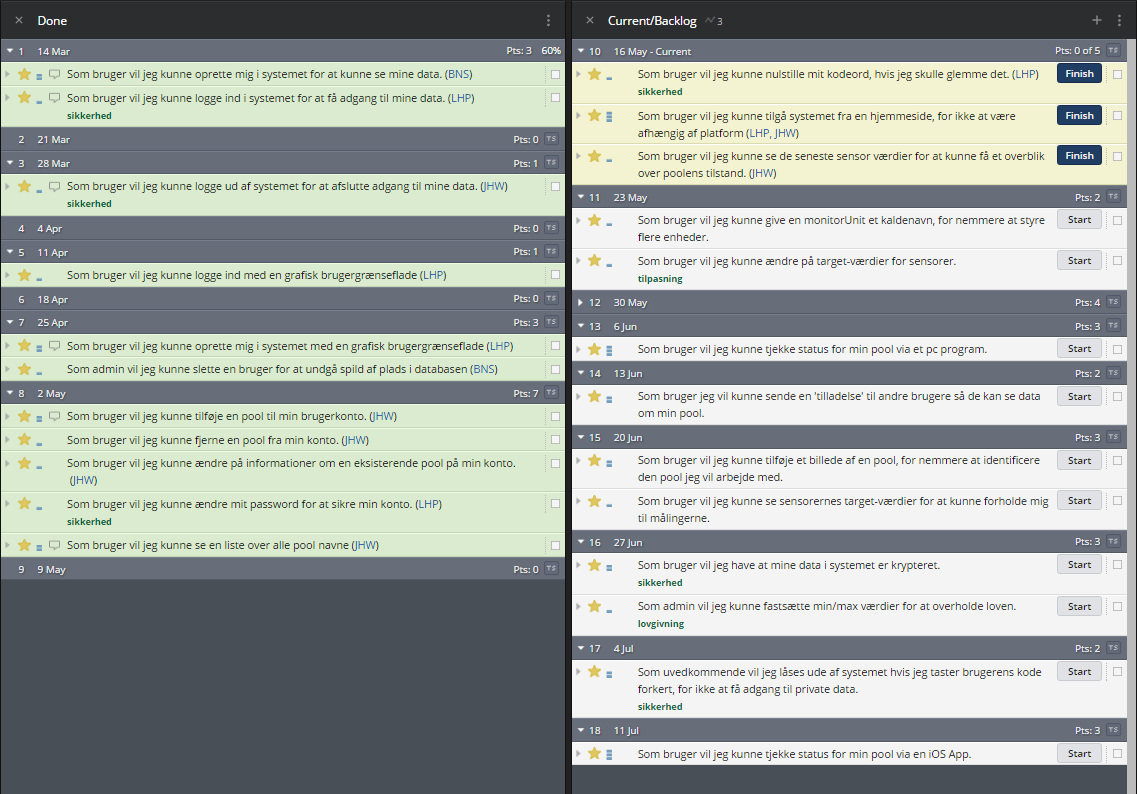
\includegraphics[width=\linewidth]{figs/processProjektGennemforsel/scrumboard.PNG}
	\caption{Pivotal tracker's interaktive scrumboard}
	\label{fig:scrumboard}
\end{figure}

 User stories er meget generelle og forklarer slutbrugers perspektiv, så det var en hjælp for gruppen at dele user stories op i mindre task - typisk specifik til den respektive undergruppes arbejde. 

\begin{figure}
	\centering
	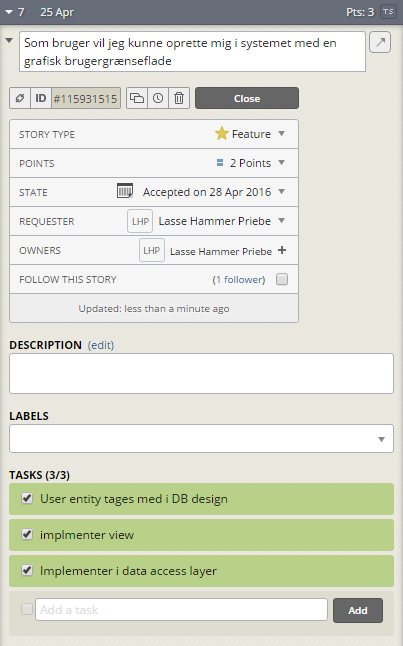
\includegraphics[width=0.5\linewidth]{figs/processProjektGennemforsel/userstory_with_tasks.PNG}
	\caption{User Story - Opret Bruger}
	\label{fig:userstory_with_tasks}
\end{figure}

Som det ses på figur~\ref{fig:userstory_with_tasks} giver Pivotal Tracker mulighed for at tjekke tasks af efterhånden som de udføres. Når alle tasks i den pågældende user story er tjekket, så trykkes Deliver, herefter kan en ny story påbegyndes. 

Start af nye user stories eller tasks sker ved et sprint planlæggende møde. For at sikre at arbejdsbyrden er passende for sprinten, vurderes hver user story af alle medlemmer. Hvert medlem vurderer på en skala fra 1-3. Et gennemsnit afgører suverænt gruppens estimering af arbejdsbyrden. Efter hvert sprint opgøres det, hvor mange point gruppen har lavet i løbet af sprinten. Antallet af point er lig med gruppens hastighed. Ved planlægning af et nyt sprint vurderes det, om gruppen kan arbejde med samme hastighed, eller højere eller lavere, hvorefter arbejdsbyrden planlægges herefter. User stories som giver meget værdi for kunden udvælges først. Værdivurderingen er en MoSCoW analyse, hvor det kvalitativ vurdereres, hvor stor værdi de respektive user stories har, ved at stemple dem med Must, Should, Could og Won't. De sorteres fra høj til lav værdi. Gruppen vurderede, at bruger skal kunne logge ind i systemet, som værende en af de vigtigste user stories, og den fik dermed et 'Must'. Den user story blev den første "spike" i den agile udvikling af Smartpool.  

\section{Test}
Sidste led i udviklingen af en del-feature er test. Det gælder for alle lag af projektet, dog adskiller måden at teste sig i de forskellige lag. GUI blev testet ved en kvalitativ test af en udvikler. Til Business logikken er klassernes metoder unit testet. Til det anvendes et automatiseret test framework Nunit, som fungerer som dokumentation af koden dvs. ændres noget i koden og testen stadig går godt, antages ændringen at være korrekt. Hvad med database??\todo{Test. Hvad med database?}

\subsection{Test Driven Development}
TDD er en udviklingsmetode, som foreskriver at test skrives før selve produktionskoden \cite{osherove2015art}. Gruppen har ikke brugt TDD 100\% gennem forløbet. 
Dog har TDD været særligt brugbart i udviklingen af DAL\footnote{Data Access Layer} laget, idet at de enkelte methoder har været enkle nok, til der kunne skrives test før selve produktionskoden skulle skrives.

Integrationstest af klasser\todo{Skriv noget om integrationstest}

\subsection{Spikes} %integration af lag?
Spikes blev i projektet brugt til at teste login funktionaliteten fra ende til anden af systemet. Brugeren logger ind gennem et GUI, hvorefter systemet forespørger database om brugeren eksisterer, og slutteligt bekræftes det, at brugeren er logget ind. Designet af systemet testes hermed fra ende til anden. Integration af systemet fra ende til anden foretages kontinuerligt langt frem med udviklingsprocessen. Det er gjort for hele tiden at teste, om arbejdet er på vej i den rigtige retning. Fejlene der opstår i første spike tages i mente, når næste Spike skal udarbejdes. 

\begin{figure}
	\centering
	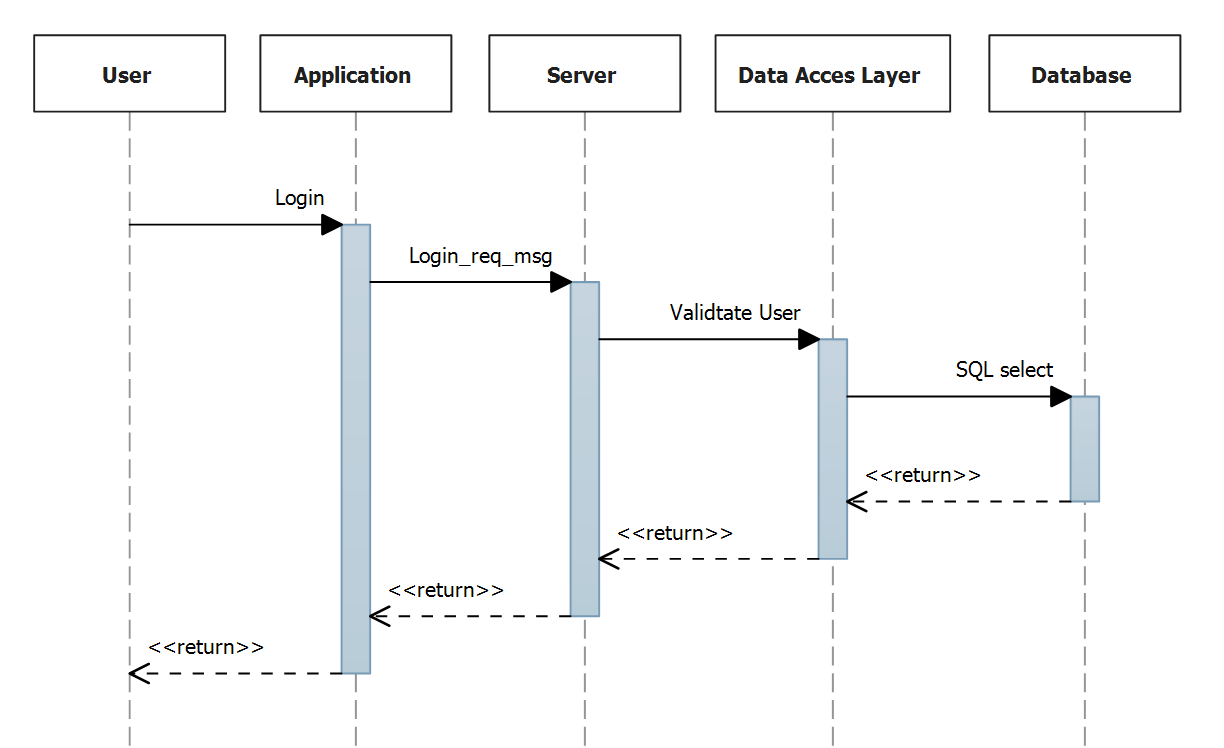
\includegraphics[width=0.9\linewidth]{figs/processProjektGennemforsel/Spike.PNG}
	\caption{Design Spike}
	\label{fig:design_spike}
\end{figure}

\section{Versionsstyring}
Softwareudviklingen er versionsstyret, for at flere udviklere kan arbejde parallelt på et projekt uden at skabe konflikter når ændringer gemmes. Til formålet har gruppen benyttet versionsstyringsværktøjet Git.

\subsection{Git} \todo{Meget indforstået}
Git bruges i projektet til al source kode, og hver feature udvikles på sin egen "branch" for at undgå konflikter. Når en feature er færdig udstedes et pull request, hvorefter repository administratoren kan merge koden ind på master branch.

For at holde styr på branches og versioner er der brugt Feature Branching \cite{atlassian2016}. Dette indebære der ikke foregår noget produktionsarbejde på master branchen. I stedet skal der oprettes en branch specielt til denne feature. Så når denne feature er testet med seneste udgave af master branchen, kan ændringerne blive "merged" eller flettet ind. På denne måde har gruppen hele tiden haft en fungerende produkt at vise frem, hvis det skulle blive nødvendigt.

\subsubsection{GitHub}
Github er online hosting af Git repositories, og er brugt i projektet til at gemme source kode, samt administrere projektets repository. I forbindelse med projektstyring og adminitration, har git været brugt til eksempelvis at tracke teamets effektivitet og commit-frekvens dvs. hvor ofte kode merges ind på master branchen.

\subsection{Travis CI og Jenkins} 
Gruppen har undervejs forsøgts sig med både med Travis CI og Jenkins. Travis er væsentlig bedre til at integrere med Github, så det bliver brugt i projektet.
Begge værktøjer er til continuos integration. CI er belejligt idet en ekstern server står for at bygge al source kode der bliver pushet til projektets repository og kører tilsvarende tests.

Dette er især nyttigt til større projekter, hvor lokale test på udviklerens computer ikke er hensigtsmæssige af tidsmæssige årsager. Travis CI er gratis til offentlige repositories på GitHub. Dog er Travis CI kun "community supported" for C\# kode \cite{communitysupportedlanguages2016}, hvilket introducerede en udfordring.

Da projektet både indeholder en applikation til PC, iOS og en web applikation, har det været en udfordring at benytte et continous integration værktøj.
Det kombineret med at hele testsuiten hurtigt kunne eksekveres lokalt, ledte til at gruppen valgte at prioritere tid brug på udvikling og lokale test.

Et forsøg med Travis skulle konstatere, om der skulle bruges mere tid på Travis CI. 
Det lykkedes at sætte github repositoriet op til kun at tillade et merge, hvis koden kan bygge og består alle tests som vist på figur~\ref{fig:travisgithubsuccess}.
Det besværliggjorde delingen af fremskridt mellem gruppens medlemmer, og blev fjernet igen.
Travis har kørt tests efter opsætningen, men det er fravalgt.

\begin{figure}[h]
	\centering
	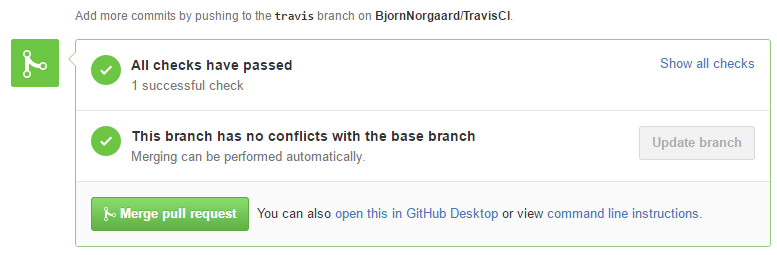
\includegraphics[width=0.8\linewidth]{figs/processProjektGennemforsel/travis/travisgithubsuccess}
	\caption{Github pull request, efter at alle test er kørt med Travis CI.}
	\label{fig:travisgithubsuccess}
\end{figure}

\section{Software test}
Software testing har været en stor del af dette projekt. Der har været stor fokus på robusthed. Der er i alt skrevet cirka 200 automatiserede tests, se figur~\ref{fig:vsUnittest}. Af disse er lidt over halvdelen skrevet til DAL, som er den mest oplagte del at enhedsteste, da eksempelvis GUI laget hovedsageligt er testet visuelt.

\begin{figure}[h]
	\centering
	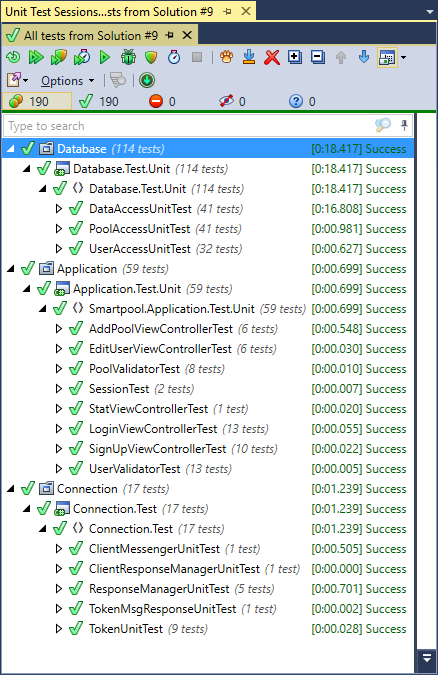
\includegraphics[width=0.5\linewidth]{figs/processProjektGennemforsel/vsUnittest}
	\caption{Unitest session i Visual Studio}
	\label{fig:vsUnittest}
\end{figure}

\subsection{NUnit- og testframeworks}\todo{Afsnittet skal muligvis flyttes til Udviklingsværktøjer...}
Et oplagt værktøj til softwaretest har været Nunit idet det bruges i vid udstrækning i forbindelse med kurset Software Test.